\documentclass[conference]{IEEEtran}

\usepackage[numbers]{natbib}
\usepackage{listings}
\lstset{breaklines}
\usepackage{hyperref}
\usepackage[outputdir=out]{minted}
\usepackage{fontspec}
\usepackage{graphicx}
\graphicspath{ {images/} }


%% Set up autoref names
\renewcommand{\sectionautorefname}{Section}
\renewcommand{\subsectionautorefname}{Section}
\renewcommand{\subsubsectionautorefname}{Section}

% correct bad hyphenation here
\hyphenation{op-tical net-works semi-conduc-tor}


\begin{document}
%
% paper title
% Titles are generally capitalized except for words such as a, an, and, as,
% at, but, by, for, in, nor, of, on, or, the, to and up, which are usually
% not capitalized unless they are the first or last word of the title.
% Linebreaks \\ can be used within to get better formatting as desired.
% Do not put math or special symbols in the title.

\title{The Effect of Rust's Abstraction Language Constructs on Traditional Object Oriented Design Patterns}

% author names and affiliations
% use a multiple column layout for up to three different
% affiliations
\author{\IEEEauthorblockN{Viktor Holmgren}
    \IEEEauthorblockA{
        Link\"oping University\\
        Link\"oping, Sweden\\
        Email: vikho394@student.liu.se}
}

% make the title area
\maketitle

% As a general rule, do not put math, special symbols or citations
% in the abstract
\begin{abstract}
    In this paper the effects of implementing traditional object oriented design patterns in Rust are evaluated with a focus on maintainability.
    More specifically, this paper seeks to find how the Rust language, which has no concept of classes nor inheritance, affect the implementation of the Adapter, Template method and Builder patterns as measured by a set of software quality metrics.
    The results are three fold:
    First, that the implementations only differ marginally compared to those written in the traditional object oriented language Java in terms of the software metrics used.
    Second, that the abstraction language constructs in Rust, specifically \emph{Traits}, have some decisive advantages and disadvantages over traditional object oriented constructs.
    Third, that the software metrics as used in this paper, are problematic when comparing languages which differ considerably in their fundamental design and paradigm support.
\end{abstract}

\IEEEpeerreviewmaketitle

\section{Introduction}
As software systems grows, so does the need for appropriate design which allows for easy handling of existing code, and the flexibility to extend the code base with new features.
Over the years similar problems have been met by different people, and different solutions have been implemented to varying degrees of success.
Those solutions which have have stuck around and have been codified, are often referred to as, \emph{design patterns}.
The actual effect of design patterns on maintainability of software are still unclear according to \citet{zhang2012:pattern-effectiveness} as it depends on a number of different factors. 
One factor which should not be overlooked is the language features which are used in implementation.

Many design patterns revolve around the Object Oriented Programming (\emph{OOP}) paradigm.
That is not surprising since the OOP paradigm sees extremely wide spread usage, with many of the most popular languages around using it as their main paradigm.
In fact, four of the five most popular programming languages in 2017 support OOP in the traditional sense, with classes and class based inheritance~\cite{ieee:lang_usage}.

As new languages emerge there is a interest for transferring knowledge, experience and even design patterns from existing languages to new ones.
Therefor one might ask one self how the utility of design patterns is impacted when they are implemented in a language which lacks any traditional OOP language constructs, such as inheritance or even classes?
Is it simply the case that these languages provide similar language features but with different terminology?
Can the different language constructs be combined to achieve an equivalent result?
Does entire new patterns emerge from the specific problems faced in the language?
Or does some patterns have no real equivalent, are there language features which remove the need for them entirely?

This paper seeks to answer how the Adapter, Template method, and Builder design patterns are affected by being implemented in the programming language Rust as measured by the software quality metrics: Design Size in Classes and Interfaces (\emph{DSCI}), Depth of Inheritance Tree (\emph{DIT}) and Coupling Between Objects (\emph{CBO}).
The Java programming language will serve as a base line for comparison of the implementations, as well as a basis for a general discussion on the maintainability effects of the language constructs available in Rust.
The reason behind choosing Adapter, Template method and Builder respectively were that:
First, Rust allows for implementation of interfaces for existing types.
Second, Rust has no concept of class based inheritance.
Third, Rust does not support function or method overloading.

%The three patterns chosen for examination are Adapter, due to the fact that Rust allows for implementation of interfaces for existing types, Template method, since Rust has no concept of class inheritance, and Builder, because Rust does not support overloading.

%The focus in the examination will be on the maintainability of the source code as measured by a number of different software quality metrics: Design size in Classes and Interfaces (\emph{DSCI}), Depth of Inheritance tree (\emph{DIT}) and Coupling between Objects (\emph{CBO}) and a general evaluation on the impact of the language constructs used.

\section{Background}

\subsection{Software Metrics}
\label{sub:software_metrics}
To make it possible to evaluate the implementations in Rust using the object oriented software metrics described, the equivalent of a class and inheritance in Rust needs to be defined since those concepts are not modeled directly.

A class as defined by \citet{gamma1993:gof} is a construct which  ``...specifies the object's internal data and representation and defines the operations the object can perform``.
In Rust this would be equivalent to a struct or enum and all implementations for that data, i.e all implementation blocks.
This would include default implementations for the concrete type as well as all trait implementations.

Rust does not have the traditional notion of class based inheritance.
It does however support inheritance for traits, sometimes called trait bounds, which fill a very similar role to an interface in most languages.
They allow for a trait to specify that another trait must also be implemented.
Therefor hierarchies can be modeled, but only leaves in a hierarchy tree can be concrete types that can instantiated.
For this paper inheritance of default methods from a trait will be considered equivalent to class inheritance as it is the closest to class based inheritance that is possible to achieve.
This does not make a trait with default methods a class however, since it neither specifes any internal data nor defines operations, it only specifies them.

The three software quality metrics that will be used in this paper are:
\begin{itemize}
    \item
        \emph{Design Size in Classes and Interfaces} (DSCI): which is the total number of classes and interfaces present in the design.
        Lower values are generally preferred since larger software size often implies increased effort when maintaining the software~\cite{riaz2009:systematic}.
    \item
        \emph{Depth of Inheritance Tree} (DIT): the level number for a class in an inheritance hierarchy.
        Base classes are defined to have a DIT of 0.
        Lower values are preferred, since deeper trees implies greater design complexity.
        Furthermore, classes deep in class hierarchies will likely inherit more methods thus making their behavior more unpredictable for the reader~\cite{kemerer:metrics}.
    \item
        \emph{Coupling Between Objects} (CBO): is the number of other classes to which a class is coupled.
        High coupling between classes is unwanted, and in turn also high CBO values, because it works against modular design and reuse of code.
        Also, a high CBO value would indicate that the class is sensitive to changes made in related classes, resulting in reduced maintainability~\cite{kemerer:metrics}.

\end{itemize}

The DSCI value is calculated on the entire implementation, whereas DIT and CBO are calculated on class level.
As implementation wide values are needed, averages over all classes will be used for DIT and CBO.

\subsection{Adapter Pattern}
\label{sub:adapter_pattern}
The Adapter design pattern as defined by \citet{gamma1993:gof} is a pattern which seeks to solve the problem of converting the interface of one or more classes into another interface which a client expects.
It can be seen as wrapping one or more existing classes with a new interface.
One common use case for this pattern is when there is a need to reuse some type of legacy component but that component does not satisfy the interface needed.

The very simple example which will be considered in this report is the following.
Suppose there is a legacy class \emph{Rectangle} which can be displayed using coordinates for the upper left corner, width and height, but the client wishes to handle a Rectangle as an instance of Shape, where Shape is an interface containing a more general display method which instead takes coordinates for the upper left corner and the bottom right.
See \autoref{fig:adapter-uml} for an UML diagram of the Adapter pattern applied to the example.

\begin{figure}[htpb]
    \centering
    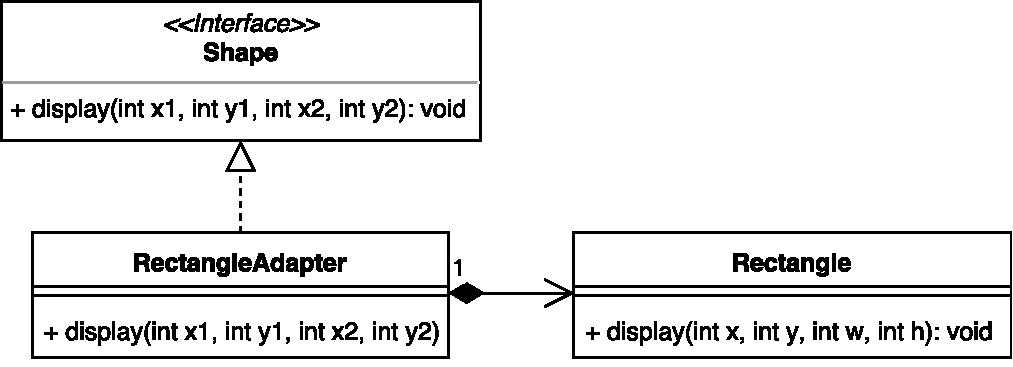
\includegraphics[width=0.8\linewidth]{adapter-ex.pdf}
    \caption{UML diagram over the Adapter example used}
    \label{fig:adapter-uml}
\end{figure}

\subsection{Template method Pattern}
\label{sub:template_method_pattern}
In the Template method pattern one defines a skeleton of an algorithm, but deferring some steps to subclasses.
It solves a similar problem as the Strategy pattern, although Strategy relies on composition rather than inheritance.
The primary use case for the Template method pattern is to reduce duplicated code between two or more classes that have much in common in terms of source code, but differ in some details ~\cite{gamma1993:gof}.

Consider the following example in which there exists several different animal classes: Cat, Sheep, et cetera, which all have a unique name and make a unique noise.
Suppose that all these animals share a \emph{what\_does\_it\_say} method which prints the animal's name and the noise they make.
The client does not want to have to care of the exact animal on which it calles the \emph{what\_does\_it\_say} method.
For simplification, only the Sheep animal will be considered.
See \autoref{fig:template-method-uml} for an UML diagram of Template method applied to the example.

\begin{figure}[htpb]
    \centering
    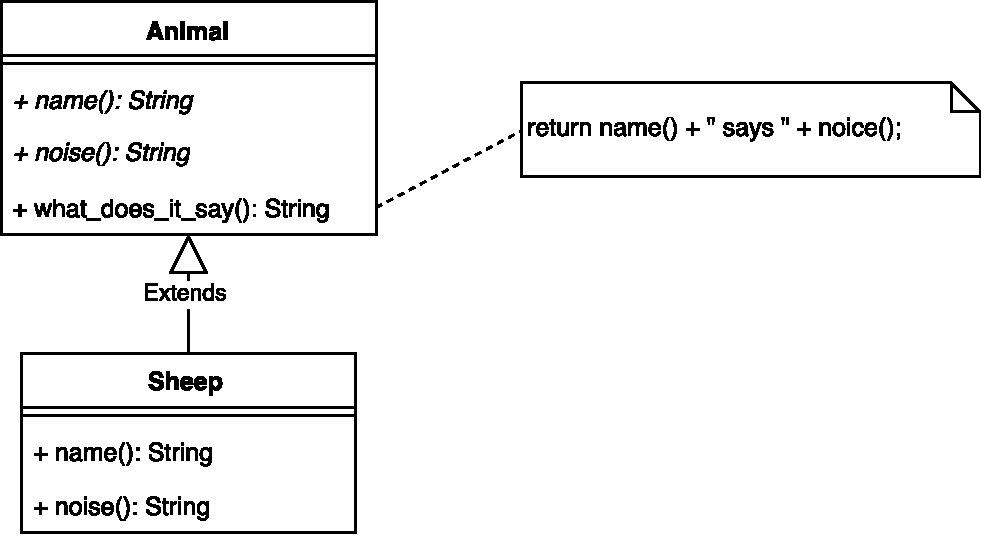
\includegraphics[width=0.8\linewidth]{template-method-ex.pdf}
    \caption{UML diagram over the Template method example used}
    \label{fig:template-method-uml}
\end{figure}

\subsection{Builder Pattern}
\label{sub:builder_pattern}

The Builder design pattern's primary intent is to reuse the same construction process to create multiple different representations by separating the construction of a complex object from its representation.
It can for example be used to avoid a rapidly expanding set of constructors on a complex object.
By separating the creation to separate class, a Builder, from the object itself the complexity of the original class is reduced~\cite{gamma1993:gof}.

The example which will be used in this paper is the following.
Suppose there exists some Process class which is rather complex, especially its constructor.
Furthermore, the client wishes to use some simplifyed method for creating Processes with many different values.
For an UML diagram depicting the Builder pattern applied to the example, see \autoref{fig:builder-uml}.

\begin{figure}[htpb]
    \centering
    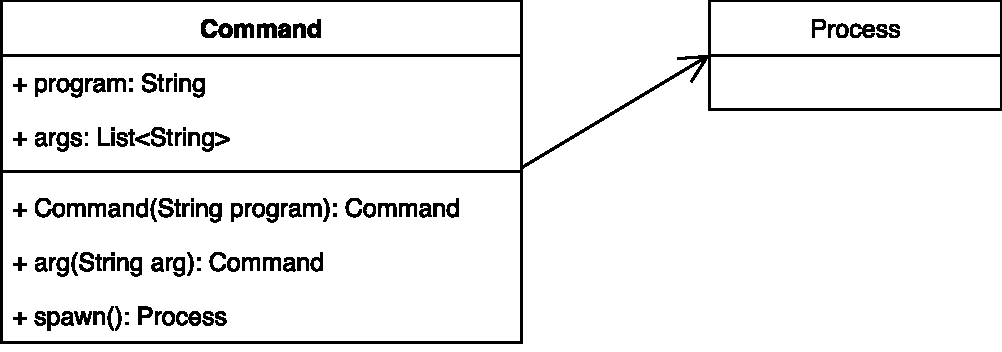
\includegraphics[width=0.8\linewidth]{builder-ex.pdf}
    \caption{UML diagram over the Builder example used}
    \label{fig:builder-uml}
\end{figure}

\subsection{Rust}
\label{sub:rust}
The Rust programming language is a relatively new language, only started in 2006 by Gradon Hoare.
Since then the project has been primarily backed by the Mozilla Foundation~\cite{rustorg2017:faq}.
Rust is a system level programming crafted for performance and critical systems.
One of its primary features it is that it guarantees memory safety without any run-time overhead, even over multiple threads~\cite{matsakis:2014:rustlang},~\cite{reed2015:proof}.
Otherwise the language tries to solve problems where languages like C++ currently are most common.

\emph{Traits} are the main way to express abstractions in Rust, and on the surface they are very similar to what would be called an \emph{Interface} in most other languages.
Similar to interfaces they allow the programmer to specify methods with arguments and return values for yet to be implemented types.
When those types are later created, they must implement all methods with the given signatures in order to satisfy the interface.
There are however some key differences between traits and typical interfaces in other languages~\cite{rustblog2015:traits}:

\begin{itemize}
    \item
        Traits can not only require methods to be implemented, but can also provide default implementations. This allows traits to fill a role similar to abstract classes.
        Note that Java added support for default methods in interfaces as well in version 8~\cite{oracle:java_default}.
    \item
        Traits can not only be implemented for new user level types, but also for existing types as trait implementation is completely separate from the type declaration.
    \item
        Traits can require constants to be specified as well as methods.
    \item
        Traits can both be statically and dynamically dispatched.
\end{itemize}

\emph{Polymorphism} is the language construct which allows for a single interface to represent multiple different types~\cite{bjarne:polymorphism}.
In Rust polymorphism is achieved using traits, and it comes both in form of static dispatch and dynamic dispatch.

For static dispatch Rust uses generics which are very similar to the way C++ templates work, i.e the compiler will instantiate multiple versions of the function for each unique type satisfying the generic bounds.
This means that generics results in zero abstraction overhead.

There is also support for dynamic dispatch, i.e dispatch at run-time when indirection is really needed, for instance when operating on a list of elements of one trait type but of varying concrete types.
Generics would not work in this case since the concrete types are different.
It is also not possible to pass traits as values to methods as the compiler generally need to know the exact size of parameter list for functions/methods and the size of a trait is unknown.
To enable dynamic dispatch values must either be \emph{Boxed}, which is done by wrapping the value in an unsized reference called a \emph{Box}, or by passing the value as a reference~\cite{rustblog2015:traits}.
See \autoref{fig:dispatch-impl} for an example on traits in Rust.
\begin{figure}[ht]
    \begin{minted}[autogobble, breaklines=true]{rust}
        trait Animal {
            /// Methods to be implemented
            fn name(&self) -> &'static str;
            fn noise(&self) -> &'static str;
        }

        // All FlyingAnimals must implement Animal, inheriting of traits
        trait FlyingAnimal: Animal {};

        /// Static dispatch: generic function, compiler will instantiate concrete functions for each caller, e.g. Sheep, Cat etc
        fn what_does_it_say<T: Animal>(animal: &T) {
            println!("{} goes {}", animal.name(), animal.noise());
        }
        /// Dynamic dispatch: Use Box pointer reference
        fn what_does_it_say2(animal: &Box<Animal>) {
            println!("{} goes {}", animal.name(), animal.noise());
        }

    \end{minted}
    \caption{Trait examples in Rust}
    \label{fig:dispatch-impl}
\end{figure}



\section{Results}
The \emph{Adapter} implementation for the example used in \autoref{sub:adapter_pattern} in the Rust programming language can be seen in \autoref{fig:adapter-impl}.
Here the implementation uses the fact that Rust allows for the implementation of traits for existing types, meaning that the \emph{Shape} trait can be implemented directly onto the \emph{Rectangle} type after it is defined.
In contrast, our Java implmenetaion requires a wrapper class to be used, \emph{RectangleAdaper}, which implements the \emph{Shape} interface and also contains a \emph{Rectangle} instance to which it forwards calls to.

The Java implementation, see \autoref{fig:adapter-java-impl}, resembles the UML diagram presented in \autoref{sub:adapter_pattern} very closely, unlike the Rust implementation which forgoes the need for an actual adapter class entirely.
As such the Rust introduced one new interface (trait) but no new classes unlike Java which introduced both a new interface, and a new class.
The use of an internal reference needed in the adapter class to forward requests in the Java implementation results in a higher a CBO value of 1 instead of 0.
The derived software metrics for the implementations can be seen in \autoref{tab:adapter-metrics}.

\begin{table}[hbtp]
    \centering
    \caption{Software metrics for Adapter implementation}
    \label{tab:adapter-metrics}
    \begin{tabular}{lllll}
        & DSCI   & DIT  & CBO   &  \\
        Rust & 2 & 0    & 0     &  \\
        Java & 3 & 0    & 1     &  \\
    \end{tabular}
\end{table}

For the \emph{Template method} implementation in Rust, seen in \autoref{fig:template-impl}, Rust's notion of default methods in traits are used to establish the shared behavior between different concrete Animals.
The other methods, \emph{name} and \emph{noise}, are not given any default implementation and therefor has to be implemented by the concrete types such as \emph{Sheep}.
In Java, see \autoref{fig:template-java-impl}, an abstract class is used to represent the Animal trait, letting the \emph{name} and \emph{noise} be abstract methods to be implemented by \emph{Sheep} which is  a concrete class extending \emph{Animal}.
The metrics calculated from the implementations can be seen in \autoref{tab:template-metrics}.
Note that the Rust implementation has a higher DIT value since the trait having the default implementation does not count as a class, i.e only the leaves in the hierarchy gets counted.

% Should CBO really be 1???
\begin{table}[hbtp]
    \centering
    \caption{Software metrics for Template method implementation}
    \label{tab:template-metrics}
    \begin{tabular}{lllll}
        & DSCI   & DIT  & CBO   &  \\
        Rust & 2 & 1    & 1     &  \\
        Java & 2 & 0.5  & 1     &  \\
    \end{tabular}
\end{table}

In the \emph{Builder} implementation in Rust, seen in \autoref{fig:builder-impl}, there are two concrete types: \emph{Command} and \emph{Process}.
Using the \emph{new} method instantiates a new \emph{Command} and sets the default state needed for creating a \emph{Process} instance.
Then using the \emph{arg} method the internal state can be altered.
Note that the \emph{arg} method returns a mutable \emph{Command} reference, allowing for chaining of calls together like $Command::new("ls").arg("l").spawn()$.
In the Java implementation, \autoref{fig:adapter-java-impl}, there are also two concrete classes working in an almost identical way, returning $this$ in \emph{arg} also allows for chaining.
From the implementations the metric values seen in \autoref{tab:builder-metrics} are calculated, and both implementations are indentical in terms of those metrics.

\begin{table}[hbtp]
    \centering
    \caption{Software metrics for Builder implementation}
    \label{tab:builder-metrics}
    \begin{tabular}{lllll}
        & DSCI   & DIT  & CBO   &  \\
        Rust & 2 & 0    & 1     &  \\
        Java & 2 & 0    & 1     &  \\
    \end{tabular}
\end{table}

\begin{figure}[btp]
    \begin{minted}[autogobble, breaklines=true]{rust}
        /// Legacy component to be adapted
        pub struct Rectangle;
        impl Rectangle {
            fn display(&self, x: i32, y: i32, w: i32, h: i32) {
                println!("Show rectangle at {},{} with dimensions: {}, {}", x, y, w, h);
            }
        }

        /// User facing interface to be used
        trait Shape {
            fn display(&self, x1: i32, y1: i32, x2: i32, y2: i32);
        }

        /// Append trait implementation
        impl Shape for Rectangle {
            fn display(&self, x1: i32, y1: i32, x2: i32, y2: i32) {
                Rectangle::display(self, x1, y1, x2-x1, y2-y1);
            }
        }
    \end{minted}
    \caption{Adapter implementation in Rust}
    \label{fig:adapter-impl}
\end{figure}

\begin{figure}[btp]
    \begin{minted}[autogobble, breaklines=true]{rust}
        trait Animal {
            /// Methods deferred to subtypes
            fn name(&self) -> &'static str;
            fn noise(&self) -> &'static str;

            // Trait default implementation, algorithm skeleton
            fn what_does_it_say(&self) {
                println!("{} goes {}", self.name(), self.noise());
            }
        }

        /// "Subtype" Sheep, implements the Animal trait
        struct Sheep;
        impl Animal for Sheep {
            fn name(&self) -> &'static str {
                "Sheep"
            }

            fn noise(&self) -> &'static str {
                "baaaaah!"
            }
        }
    \end{minted}
    \caption{Template method implementation in Rust}
    \label{fig:template-impl}
\end{figure}

\begin{figure}[btp]
    \begin{minted}[autogobble, breaklines=true]{rust}
        /// Builder to create a Process instance
        pub struct Command {
            program: &str,
            args: Vec<&str>,
        }

        impl Command {
            /// Constructor, set default values
            pub fn new(program: &str) -> Command {
                Command {
                    program: program,
                    args: Vec::new()
                }
            }

            /// Add an argument to pass to the program.
            pub fn arg<'a>(&'a mut self, arg: &str) -> &'a mut Command {
                self.args.push(arg);
                self
            }

            /// Executes the command as a child process, which is returned.
            /// Actually builds the instance
            pub fn spawn(&self) -> IoResult<Process> {
                ...
            }
        }
    \end{minted}
    \caption{Builder implementation in Rust}
    \label{fig:builder-impl}
\end{figure}

\begin{figure}[btp]
    \begin{minted}[autogobble, breaklines=true]{java}
        interface Shape {
            void display(int x1, int y1, int x2, int y2);
        }

        class Rectangle {
            public void draw(int x, int y, int w, int h) {
                System.out.println("Show rectangle at " + x + ", " + y + " with dimensions: " + w + ", " + h); 
            }
        }

        class RectangleAdapter implements Shape {
            private Rectangle adaptee;

            public RectangleAdapter() {
                this.adaptee = new Rectangle();
            }

            @Override
            public void draw(int x1, int y1, int x2, int y2) {
                adaptee.display(x1, y1, x2-x1, y2-y1);
            }
        }
    \end{minted}
    \caption{Adapter implementation in Java}
    \label{fig:adapter-java-impl}
\end{figure}

\begin{figure}[btp]
    \begin{minted}[autogobble, breaklines=true]{java}
        abstract class Animal {
            public abstract String name();
            public abstract String noise();

            public void what_does_it_say() {
                System.out.println(this.name() + " goes " + this.noise());
            }
        }

        // Sheep subclass, extends Animal 
        class Sheep extends Animal {
            public String name() {
                return "Sheep";
            }

            public String noise() {
                return "baaaaah!";
            }
        }
    \end{minted}
    \caption{Template method implementation in Java}
    \label{fig:template-java-impl}
\end{figure}

\begin{figure}[btp]
    \begin{minted}[autogobble, breaklines=true]{java}
        class Command {
            private String program;
            private List<String> args;

            public Command(String program) {
                this.program = program;
                this.args = new ArrayList<String>();
            }

            // Add an argument to pass to the program.
            public Command arg(String arg) {
                this.args.add(arg);
                return this;
            }

            // Executes the command as a child process, which is returned.
            // Actually builds the instance
            public Process spawn() {
                ...
            }

        }
    \end{minted}
    \caption{Builder implementation in Java}
    \label{fig:builder-java-impl}
\end{figure}

\section{Discussion}

% Discuss that the metrics are very similar
% Discuss that the traits have some key advantages and disadvantages 
% Discuss that the metrics may not be that good for measuring non object oriented languages 

From the results above we see that the implementations in Rust and Java are quite similar which is also reflected in the metrics. 
Therefor there is lettle general support from the metrics in the idea of change of maintainability of any of the solutions apart from the adapter implementation which is quite different.
There are however some key points to be discussed.

From the Adapter pattern example we see that Rust's support for implementation of traits for existing types eliminates the need for the pattern entirely.
By having trait behavior for a type be separate from the data of that type we are able to extend the functionality of existing types without effecting the existing code base.
This feature allows for great maintainability out of the box since the \emph{Open-Closed} principle is basically enforced by the langauge~\cite{gamma1993:gof}.
By allowing extention of behavior in this way we also remove the need for converting between adapters and adaptees in any mediating source code between the client, which wishes the use the adapter, and the rest of the code base, which may use the legacy component.
In Java however we would practically need to introduce a facade between the existing code base and the client which translates input of legacy instances into adaptered instances and output of adaptered instances into legacy instances.
This in turn has a great effect of maintainability since the cost of reducing existing components in Rust is minimized.

But suppose we had $N$ number of legacy components which we wanted to implement the \emph{Shape} for. 
In Java we would have introduced $N$ new adapter classes.
Where as in Rust we would have added zero new classes according to the definition given in \autoref{sub:software_metrics}, i.e the size of introducing $N$ adapter patterns would be constant.
This strange result seems to point to a flaw in the definition of a class in Rust as given in this paper.
However there are only two possible options in defining a class, both yielding unreasonable results:
\begin{itemize}
    \item The type and all implementations counts as one class.
    \item The type and default implementation counts as one class, each trait implementation constitutes an additional class.
\end{itemize}
The first definition is what is used in this paper.
By the second definition common types would make up a very large number of classes, for example the standard vector collection \emph{vec} in Rust would constitute over a hundred classes~\cite{rustdoc:vec}.
This I believe points to a more general problem of using specifically object oriented metrics for evaluating languages which are not traditionally object oriented.
I see two possible solutions to this, either to use non object oriented metrics such as number of lines of code (LOC) with the downside of not being able to reason about higher level constructs and for instance coupling easily, or to only use object oriented metrics for which no interpretations would have to be made.
This could however greatly reduce the number of available metrics when comparing certain languages.
We see a similar problem in the DIT since it in Rust, using the definition of class, only counts leaves as classes but includes traits as part of the hierarchy, unlike in Java where every node in the hierarchy is used.

Regarding the template method implementations we see strikingly similar solutions.
Traits with default implementations fills a role similar to that of an abstract class in Java and many other languages.
However, let there be known that it is not equivalent to an abstract class since a Rust trait cannot hold any state.
Therefor it becomes difficult to replicate the behavior of a more complex case of the template method, specifically when the algorithm skeleton and surrounding methods rely on state between method calls.
In this case one should probably look to the similar \emph{Strategy} pattern instead when developing in Rust, since it does not require any class based inheritance.
Furthermore one should probably prefer strategy generally over template method any way since it works based on composition rather than inheritance~\cite[p.32]{gamma1993:gof}.

Finally, the builder pattern is practically identical between the two languages, disregarding syntax differences.
Because Rust does not support function/method overloading the builder pattern becomes very useful.
Not having support for multiple constructors means that a programmer in Rust would have to create and maintain a large number of uniquely named methods that constitute different constructors, leading to poor maintainability.
Where as with a builder there is a separation of the construction and the behavior of a type thus resolving the programmer for creating variants of the "new" method and instead only adding methods when new parameters to the actual constructor is added.
It is important to note however that overloading can in some sense be achieved through trait implementations since we can over different trait implementations name our methods identically, even with the same parameter list.
Using traits does of course imply that those traits need to be created also, so it is not exactly equivalent.
Still, the builder is very useful, so much in fact that it is used multiple times in the Rust standard library and the example used in this paper is actually a simplification the \emph{Command} builder in the Rust standard library~\cite{rustdoc:command}.
There even exists Rust libraries that are able to automatically derive, i.e let the compiler generate source code, builder patterns for arbitrary types~\cite{cratesio:builder}.


% trigger a \newpage just before the given reference
% number - used to balance the columns on the last page
% adjust value as needed - may need to be readjusted if
% the document is modified later
%\IEEEtriggeratref{8}
% The "triggered" command can be changed if desired:
%\IEEEtriggercmd{\enlargethispage{-5in}}

% references section

% can use a bibliography generated by BibTeX as a .bbl file
% BibTeX documentation can be easily obtained at:
% http://mirror.ctan.org/biblio/bibtex/contrib/doc/
% The IEEEtran BibTeX style support page is at:
% http://www.michaelshell.org/tex/ieeetran/bibtex/
%\bibliographystyle{IEEEtran}
% argument is your BibTeX string definitions and bibliography database(s)
%\bibliography{IEEEabrv,../bib/paper}
%
% <OR> manually copy in the resultant .bbl file
% set second argument of \begin to the number of references
% (used to reserve space for the reference number labels box)
%\begin{thebibliography}{1}
%
%\bibliographystyle{./IEEEtran}

\clearpage
\bibliographystyle{IEEEtranN}
\bibliography{IEEEabrv,references}




% that's all folks
\end{document}
